\documentclass[letterpaper, reqno,11pt]{article}
\usepackage[margin=1.0in]{geometry}
\usepackage{color,latexsym,amsmath,amssymb,graphicx, float}
\usepackage{hyperref}

\hypersetup{
colorlinks=true,
linkcolor=magenta,
filecolor=magenta,
urlcolor=cyan,
}

\graphicspath{ {images/} }

\begin{document}
\pagenumbering{arabic}
\title{ELEC 481 Final Exam}
\date{26/06/22}
\author{Xander Naumenko (38198354)}
\maketitle

{\noindent\bf Question 1a.} For this CCA class the interest rate associate is 55\%. The first year is then $55\%\cdot \frac{1}{2}\cdot 350000=\$96250$. The other years are calculated using the following formula: 
\[
CCA_n=P (1-\frac{d}{2})(1-d)^{n-2}d
.\]
See the attached excel spreadsheet for the table. The depreciation value in year 6 is \$5723. 

{\noindent\bf Question 1b.} Using the formula for straight line depreciation, the 6th year's depreciation value is $(350000-15000) /6=\$55833$. 

{\noindent\bf Question 1c.} For 6th year: 
\[
d_t=\frac{N-t+1}{SOYD}(B-S)=\frac{1}{1+2+3+4+5+6}\cdot (350000-15000)=\$15952
.\]

{\noindent\bf Question 1d.} Using the formula (calculated in excel): 
\[
d_n=DB(1-D)^{n-1}=\$15364
.\]

{\noindent\bf Question 2a.} Using excel the net present worth of the benefits and costs were calculated. This was done by going through year by year and inputting that year's costs and benefits, then applying a discount rate of 1.07 per year. The benefit of option 1 was \$33484579 and it's cost was \$18688270, while for Option 2 the benefit was \$37192484 and cost was \$23772943. The resulting ratios were a B/C of 1.79 for option 1 and 1.56 for option 2. 

\medskip

{\noindent\bf Question 2b.} Since option 1 has the higher B/C ratio, we start that as the default best option. To see if we should switch, we can use incremental analysis. Using the different between the two's benefits and costs, we find the B/C ratio of these differences to be 0.729. Since this ratio is less than 1, it doesn't make sense to switch. 

\medskip

{\noindent\bf Question 2c.} The best option is option 1, since it has the higher B/C ratio and the incremental B/C ratio was less than 1. 

\medskip

{\noindent\bf Question 3a.} See the spreadsheet for the full table and calculations. The CCA's first year was calculated by $45\%\cdot \frac{1}{2}\cdot P$, while subsequent years are: 
\[
CCA_n=P (1-\frac{d}{2})(1-d)^{n-2}d
.\]
From this we see that the final book value is \$992843 and the asset was sold for \$2000000, so there was recaptured depreciation of \$1007157. 

\medskip

{\noindent\bf Question 3b.} See the spreadsheet for the full table and calculations or Figure \ref{fig:q3} for reference. From this we see that the final book value is \$1418347 and the asset was sold for \$1300000, so there was loss on disposal of \$118347.

\begin{figure}[htpb]
    \centering
    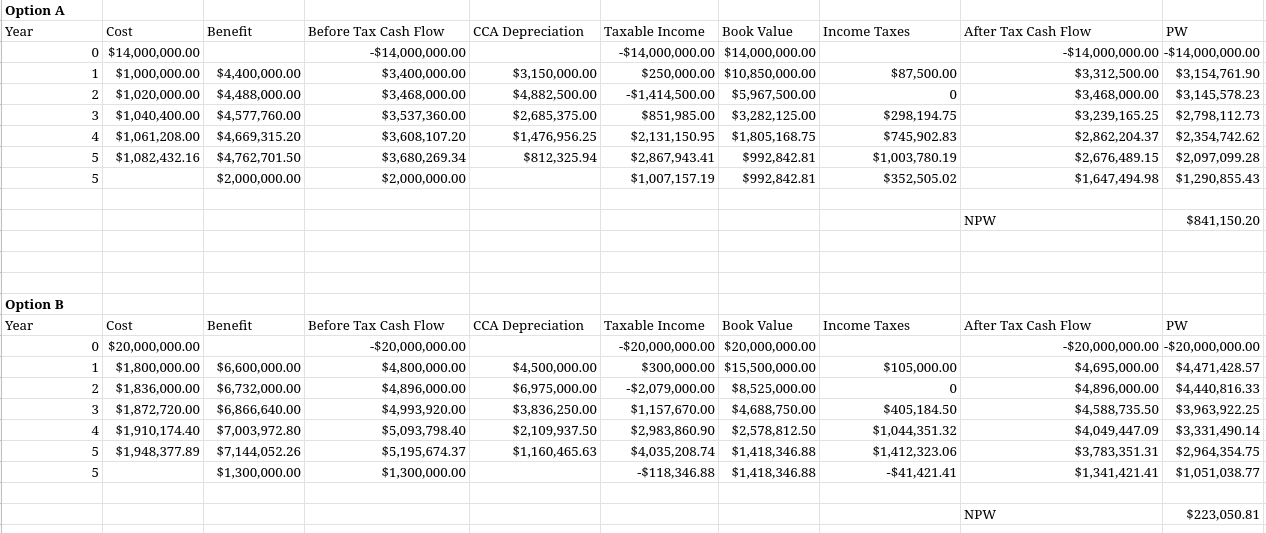
\includegraphics[width=0.8\textwidth]{q3}
    \caption{Question 3 cash flow}
    \label{fig:q3}
\end{figure}

\medskip

{\noindent\bf Question 3c.} See the attached excel spreadsheet. Note that I assume for this question, as confirmed by a Piazza post, that tax benefits do not role over to subsequent years (i.e. you can't get money from the government for taxes). The net present worth of Option A was \$1290198, while Option B had a net present worth of \$883051. 

{\noindent\bf Question 3d.} By applying the IRR function to the after tax cash flow we see that Option A has a higher IRR of 6.89\% than that of Option B of only 5.31\%, so start by assuming A is the best choice. Applying incremental IRR analysis, we compute the difference between their two net cash flows. The resulting IRR is 0.9\% which is smaller than 5\%, so it is not worth it to switch and Option A is the best due to incremental IRR analysis. 

\medskip

{\noindent\bf Question 4.} Changing borrowing interest rates would change the best option because the tradeoff of time vs. money of various options differs. The higher the borrowing rate the more that options that emphasize short term gains are favored, since money is worth more sooner. Similarly if the borrowing rate is low then options that take a long time to pay off are more feasible since money held up in an investment loses value slower. 

As a simplified example of this, consider two choices: one where you do nothing but invest the money at the borrowing rate, and another where you pay \$10 now to get \$100 ten days from now. If the interest rate was \$0 then clearly you should take the second option since you end up \$90 richer at the end of the 10 days, but if the interest rate was 100\% per day, then the do nothing option would be better since you would end up with $\$10\cdot 2^{10}=\$10240$ instead of just $\$100$. In the same way choice tables have this same tradeoff between time and money for each of their entries, although obviously not usually so pronounced. 

\medskip

{\noindent\bf Question 5.} The errors are presented with the cell they occur in in brackets (or a cell close to the error if not exactly contained in one cell): 

\begin{itemize}
    \item{(C6) Capital cost of option A is incorrectly inputted as \$170000 instead of \$190000. This is wrong since the parameters for the model don't match reality. }
    \item{(C8) Operating cost of option A is incorrectly inputted as \$40000 instead of \$80000. Same reason for being wrong as first error. }
    \item{(C10) Sales revenue of option A is incorrectly inputted as \$140000 instead of \$110000. Same reason for being wrong as first error. }
    \item{(C52) MARR of option B is incorrectly inputted as 4\% instead of 10\%. Same reason for being wrong as first error. }
    \item{(H8) First year's of CCA depreciation has a missing factor of $\frac{1}{2}$ in it for Option A. This will incorrectly cause the CCA to be much bigger than reality. }
    \item{(N9) Sales revenue for Option A doesn't increase year by year by the revenue rate increase. This would reduce the total revenue reported. }
    \item{(N45) Operating costs for Option B increase by the interest rate on loan instead of the escalation rate. This would overestimate the rate of operating expenses increase in this case. }
    \item{(V49) Recaptured CCA has an extra negative for Option B compared to Option A. This would cause the recaputed CCA to add instead of subtract and throw the total revenue off. }
    \item{(K47 by ommission) Capital asset loan repayment is omitted from Option B in the expenses section. This will mean the model won't take into account a revenue stream. }
    \item{(M24) CCA and loss/gain on disposal is double counted for Option A. This will cause money to be accounted for twice which will skew the final revenue. }
    \item{(M30) Discounted net ATCF is incorrectly calculated using the interest rate on loan for Option A instead of MARR. This confuses the two completely different percentages, since the interest rate on the loan does not necessarily equal the MARR. }
    \item{(M33) For option A, the disposal revenue is counted as a benefit while for option B it was counted as a (negative) cost. Either one of these is fine, but because they're applied differently between the two options the two B/C ratios are rendered incomparable. }
    \item{(L64) The discounted benefits and discounted costs for Option B applies the MARR of Option A instead of the MARR of Option B. This would be fine if the MARR were always the same for the two projects, but since they were specified separately the cell should use its own respective rate to enable switching in the future. }
\end{itemize}
    
\medskip

{\noindent\bf Question 6a.} See the excel spreadsheet, or Figure \ref{fig:q6} for convenience. There we see the probability distribution of the scenario for each possible combination of shifts and life. The probability was found by simply multiplying the probability of each component events together. 

\medskip

{\noindent\bf Question 6b.} Again see the excel spreadsheet or Figure \ref{fig:q6} for the net present worth for each option in the last column. This was calculated using the following formula: 
\[
NPW=-C+A(P /A, i, n)
\]
where C is the capital cost and A is the annual savings. 

\medskip

\begin{figure}[htpb]
    \centering
    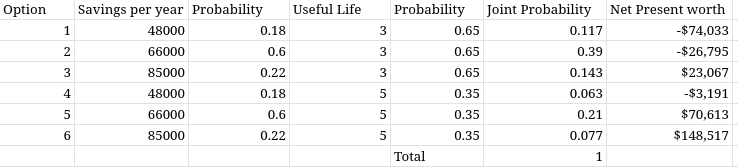
\includegraphics[width=0.8\textwidth]{q6}
    \caption{Probability distribution and NPW for question 6}
    \label{fig:q6}
\end{figure}

{\noindent\bf Question 6c.} The expected value can be calculated as the sum of the NPW times the probability of it occuring. Doing in excel results in an expected value of: 
\[
    EV=\sum_{n=1}^6 NPW_n\cdot P_n=\$10250
.\]

\medskip

{\noindent\bf Question 7a.} See the excel spreadsheet where each year's salary is calculated year by year. From this we see that the nominal salary for Job Offer 1 goes up to \$157838 and Job Offer 2 goes to \$165654. 

\medskip

{\noindent\bf Question 7b.} Real salary is found by taking the nominal salary for each year and dividing by the inflation rate to the power of the number of years (in this case the inflation only starts on year 2 as per the question though). From the spreadsheet we see that it is \$130912 for Offer 1 while it is \$151464 for Offer 2. 

\medskip

{\noindent\bf Question 7c.} Looking at the spreadsheet we see that year 6 is the first year that the real salary for Offer 2 surpasses that of Offer 1. 

\medskip

{\noindent\bf Question 7d.} Option 2 is better, since the total net present worth of the entire 10 years worth of salary (\$1319574) is higher than that of Option 1 (\$1293250). These values were calculated by simply taking the sum of all of the real salaries. 

\medskip

{\noindent\bf Question 8.} The lost interest on capital funds represents the opportunity cost of not investing the money you're using to buy the car with. This has to be included in the analysis because for the cost of the car to be worth, the total benefit must be even greater than the upfront cost. The benefit has to make up for the fact that you could have been earning interest on the money you used to buy the cars, which is represented by the opportunity cost. 

This showcases one of the key concepts of this course, the time value of money. By investing in a car over the span over many years, the money spent now has additional costs over the span of it's lifetime than just its nominal costs/benefits, which in this case is represented by an opportunity cost but it's worth noting that it could also be shown by a discount rate. 

\medskip

{\noindent\bf Question 9.} The discount rate that I would recommend the company use would depend on some of the specifics of the situation. Assuming that the company is borrowing the money to invest in the potential projects, then the most obvious rate to use as the discount rate would be the rate at which the company is borrowing the money. If the money is coming straight from the company's cash, then an appropriate discount rate would be the rate of return that the company could get through a do nothing option, whether that be investing at a bank or increasing funding for an existing project that has a well established rate of return. The principle I would apply is that of opportunity cost, as the discount rate should represent the rate of return of the next best option for each of the projects, which depending on the situation may be either investment or not borrowing the money. 

Of the candidates mentioned above I would recommend that the firm consider the candidates that best reflect how money would be spend if none of the projects are funded. For example if the company is borrowing the money, if none of the projects were funded then the money simply wouldn't be borrowed and the discount rate should reflect this. If the company has cash and could invest it then the rate of return that they would get is what should be considered as the discount rate. 

\end{document}
